\documentclass[../Chapter.tex]{subfiles}

\begin{document}

\chapter{A Special Case of Fermat's Conjecture}

\subsection*{Exercise 1.1}

The direct computation is straightforward but laborious. We use the observation that $\mathbf{N}(z)=z\ovl{z}$ whenever $z\in\ZZ[i]$. Given $\alpha,\beta\in\ZZ[i]$, then $$\mathbf{N}(\alpha\beta)=\alpha\beta\ovl{\alpha\beta}=\alpha\ovl{\alpha}\beta\ovl{\beta}=\mathbf{N}(\alpha)\mathbf{N}(\beta)$$

If $\alpha\mid\gamma$ in $\ZZ[i]$. Write $\gamma=\alpha\beta$ where $\beta\in\ZZ[i]$, then $\mathbf{N}(\gamma)=\mathbf{N}(\alpha)\mathbf{N}(\beta)$. Since $\mathbf{N}(\beta)\in\ZZ$, we have $\mathbf{N}(\alpha)\mid\mathbf{N}(\gamma)$ in $\ZZ$.

\subsection*{Exercise 1.2}

Let $\alpha\in\ZZ[i]$ be a unit, then $\alpha\mid 1$ in $\ZZ[i]$. By Ex 1.1, $\mathbf{N}(\alpha)\mid \mathbf{N}(1)=1$ in $\ZZ$. This forces $\mathbf{N}(\alpha)=1$ because from the definition of $\mathbf{N}$ we know its image is non-negative. Conversely, suppose $\mathbf{N}(\alpha)=\alpha\ovl{\alpha}=1$. This immediately implies $\alpha$ is a unit because we know $\ovl{\alpha}\in\ZZ[i]$.

It's easy to see that $\mathbf{N}(a+bi)=a^2+b^2=1$ has only four integral solutions, namely, $(a,b)=(\pm1,0),(0,\pm1)$. The corresponding elements are $a+bi=\pm1,\pm i$. So these four are units in $\ZZ[i]$.

\subsection*{Exercise 1.3}

Write $\alpha=ab$ where $a,b\in\ZZ[i]$. Suppose $\mathbf{N}(\alpha)=\mathbf{N}(a)\mathbf{N}(b)$ is a prime in $\ZZ$, then either $\mathbf{N}(a)=1$ or $\mathbf{N}(b)=1$. By Ex 1.2 we have one of $a,b$ is a unit. This means that $\alpha$ is irreducible.

Suppose $\mathbf{N}(\alpha)=\mathbf{N}(a)\mathbf{N}(b)=p^2$ for some prime $p$ in $\ZZ$. If one of $\mathbf{N}(a),\mathbf{N}(b)=1$ then we are done, so assume $\mathbf{N}(a)=\mathbf{N}(b)=p$, this is impossible because $p\equiv 3\pmod{4}$ and the $\mathbf{N}(a),\mathbf{N}(b)$, as sums of two squares, can only be $0,1,2$ mod 4.

\subsection*{Exercise 1.4}

Since $\mathbf{N}(1-i)=2$ is a prime in $\ZZ$, by Ex 1.3, $1-i$ is irreducible in $\ZZ[i]$. And from $(1-i)^2=-2i$ we get $2=i(1-i)^2$. By Ex 1.2 we know $i$ is a unit.

\subsection*{Exercise 1.5}

Note that $2+i=i(1-2i)$ and $2-i=-i(1+2i)$ and by Ex 1.2, $i,-i$ are units. So the two factorizations are in fact the same (up to units).

\subsection*{Exercise 1.6}

\subsection*{Exercise 1.7}
Let $I\neq 0$ be an ideal in $\ZZ[i]$ and take a non-zero element $\alpha\in I$ s.t. $\mathbf{N}(\alpha)$ is minimized. For each $n+mi\in\ZZ[i]$, we have $\alpha(n+mi)=n(\alpha)+m(i\alpha)$. So $$(\alpha)=\alpha\cdot\ZZ[i]=\{n(\alpha)+m(i\alpha)\mid n,m\in\ZZ\}$$

We put $\alpha$ in the fourth quadrant as an example. The other situations are very similar.

\begin{center}
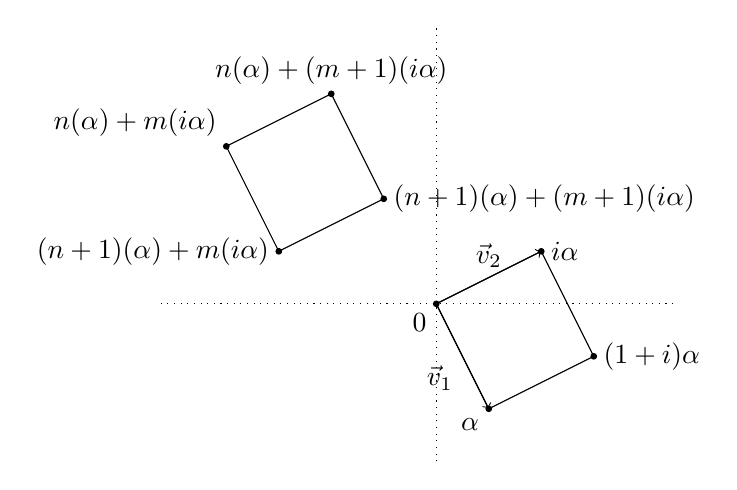
\begin{tikzpicture}
\draw[dotted] (-3.5,0)--(3,0);
\draw[dotted] (0,-2)--(0,3.5);

\coordinate (A) at (0,0);
\coordinate (B) at (1/1.5,-2/1.5);
\coordinate (C) at (2/1.5,1/1.5);
\coordinate (D) at (3/1.5,-1/1.5);
\filldraw (A) circle (1pt) node[below left] {$0$}
-- (B) circle (1pt) node[below left] {$\alpha$}
-- (D) circle (1pt) node[right]  {$(1+i)\alpha$}
-- (C) circle (1pt) node[right]  {$i\alpha$}
-- (A);

\draw[->] (A) -- (B) node[midway, below left] {$\vec v_1$};
\draw[->] (A) -- (C) node[midway, above] {$\vec v_2$};

\coordinate (A') at (-4/1.5,3/1.5);
\coordinate (B') at (1/1.5-4/1.5,-2/1.5+3/1.5);
\coordinate (C') at (2/1.5-4/1.5,1/1.5+3/1.5);
\coordinate (D') at (3/1.5-4/1.5,-1/1.5+3/1.5);
\filldraw (A') circle (1pt) node [above left] {$n(\alpha)+m(i\alpha)$}
-- (B') circle (1pt) node[left] {$(n+1)(\alpha)+m(i\alpha)$}
-- (D') circle (1pt) node[right]  {$(n+1)(\alpha)+(m+1)(i\alpha)$}
-- (C') circle (1pt) node[above]  {$n(\alpha)+(m+1)(i\alpha)$}
-- (A');

\end{tikzpicture}
\end{center}
As the graph above illustrates, when $n,m$ run through all integers, these squares will cover the whole complex plane. Note that all the vertices are indeed in $(\alpha)$.

Clearly we have $\{\text{vertices}\}=(\alpha)\subseteq I$. If $(\alpha)\varsubsetneq I$, then $\exists r\in I,r\notin(\alpha)$. So we know $r+c\cdot\alpha,r+d\cdot i\alpha\in I$ for all $c,d\in\ZZ$. Note that for $z\in\CC$, $z+\alpha$ and $z+i\alpha$ means $z$ moving toward the direction $\vec v_1$ and $\vec v_2$ for the distance equals the side length of the squares, respectively. (Also note that minus sign will mean the opposite direction.) This shows geometrically that $z$ can get closer to the origin than $\alpha$, i.e., $\mathbf{N}(z)<\mathbf{N}(\alpha)$, after walking enough steps (choosing $c,d$ accordingly). And since $z\notin(\alpha)$, $z$ is not one of the vertices. This means $z$ will not arrive at the origin, i.e., the resulting number won't be zero. This contradicts to the selection of $\alpha$. So we may now conclude that $I=(\alpha)$ is principal.
 
\subsection*{Exercise 1.8}

(a) Write $\ZZ/p\ZZ=\langle a \rangle=\{a,a^2,a^3,\ldots,a^{p-1}=1\}$. It's easy to see that $a^{(p-1)/2}\equiv -1 \pmod{p}$. Take $n=a^{(p-1)/4}\in\ZZ$, then $n^2\equiv -1\pmod{p}$.

(b) If $p$ is irreducible in $\ZZ[i]$, by Ex 1.7, $\ZZ[i]$ is a PID. So $p$ is also a prime element in $\ZZ[i]$. By (a), $p\mid n^2+1=(n+i)(n-1)$ for some $n\in\ZZ$. So $p\mid n+i$ or $p\mid n-i$. In the former case, $\exists \alpha\in\ZZ[i]$ s.t. $n+i=p\alpha$. But it's easy to see that the multiple of $p$ and an element in $\ZZ[i]$ can not be $n+i$. (Just consider the imaginary part.) This leads to a contradiction. The latter case is similar.

(c) By (b), $p=(a+bi)(c+di)$ where $a+bi,c+di$ are non-units. By taking norms we have $p^2=(a^2+b^2)(c^2+d^2)$. None of the terms on the right is $1$, so they must be $p$. Hence, $p=a^2+b^2=c^2+d^2$ is a sum of two squares.

\subsection*{Exercise 1.9}

Let $x=a+bi\in\ZZ[i]$. For the case $a\neq 0,b=0$. (So $x=a$ is real.) If $a=\pm2$ then by Ex 1.4, $a$ is not irreducible. If $|a|\equiv 1\pmod{4}$ is a prime then by Ex 1.8(b), $a$ is not irreducible. If $|a|\equiv 3\pmod{4}$ is a prime then by Ex 1.3, since $\mathbf{N}(a)=a^2$, $a$ is irreducible. Clearly, $a$ is not irreducible if $a$ is composite. On the other hand, the case when $a=0,b\neq 0$ is similar. Hence, we have the following:

$x=a\in\ZZ[i]$ is irreducible iff $|a|\equiv 3\pmod{4}$ is a rational prime. And $x=bi\in\ZZ[i]$ is irreducible iff $|b|\equiv 3\pmod{4}$ is a rational prime.

Now, assume $a,b\neq 0$. We claim that $a+bi$ is irreducible iff $\mathbf{N}(a+bi)=a^2+b^2$ is a rational prime. Recall that $(\Leftarrow)$ has already been proven in Ex 1.3.

$(\Rightarrow)$ Suppose $a+bi$ is irreducible. We may assume $a+bi\not\sim 1+i$ because this case is easy. Since we know from Ex 1.7 that $\ZZ[i]$ is a UFD, by factoring $a^2+b^2$ in $\ZZ$, we may write $(a+bi)(a-bi)=a^2+b^2=(a+bi)(c+di)(\jk)$ where $(a+bi)(c+di)$ is a rational prime $p$ of the form $4k+1$. (We know $p$ is of the form $4k+1$ and not $4k+3$ is because we've already shown that rational prime of the form $4k+3$ is irreducible. Note also that we indeed need the assumption that $a,b\neq 0$.) This means $a^2+b^2=c^2+d^2=p\equiv1\pmod{4}$ by Ex 1.8(c) and so we are done.

\subsection*{Exercise 1.10}

Write $$a+b\omega=a+b\left(\frac{-1}{2}+\frac{\sqrt{3}}{2}i\right)=\left(a-\frac{b}{2}\right)+\left(\frac{\sqrt{3}b}{2}\right)i=u+vi$$ where $u,v\in\RR$. Then $$u^2+v^2=\left(a-\frac{b}{2}\right)^2+\left(\frac{\sqrt{3}b}{2}\right)^2=a^2-ab+\frac{b^2}{4}+\frac{3b^2}{4}=a^2-ab+b^2=\mathbf{N}(a+b\omega)$$

\subsection*{Exercise 1.11}

See Ex 1.1 for analog.

\subsection*{Exercise 1.12}

Let $\alpha\in\ZZ[\omega]$ be a unit, then $\alpha\mid 1$ in $\ZZ[\omega]$. By Ex 1.11, $\mathbf{N}(\alpha)\mid \mathbf{N}(1)=1$ in $\ZZ$. This forces $\mathbf{N}(\alpha)=1$ because by Ex 1.10 we know the image of $\mathbf{N}$ is non-negative. Conversely, suppose $\mathbf{N}(\alpha)=\alpha\ovl{\alpha}=1$. This immediately implies $\alpha$ is a unit because we know $\ovl{\alpha}\in\ZZ[\omega]$.

Consider $\mathbf{N}(a+b\omega)=a^2-ab+b^2=1$. WLOG, assume $|a|\geq|b|\geq0$. By a simple calculation it's easy to see that $(a,b)=(\pm1,0),(0,\pm1),(1,1),(-1,-1)$ are all of the integral solutions when $|b|\leq1$. The corresponding elements are $\pm1,\pm\omega,\pm\omega^2$. So these six are units in $\ZZ[i]$.

It's remaining to show $a^2-ab+b^2=1$ has no integral solutions when $|b|\geq 2$. This follows easily when $ab<0$, i.e., they have the different signs. So assume $a,b$ are both positive or both negative. In this case we have $|ab|=|a||b|=ab$. Now the result follows by the observation that $$a^2-ab+b^2=|a|^2-|a||b|+|b|^2=|a|(|a|-|b|)+|b|^2\geq |b|^2\geq 4$$

\subsection*{Exercise 1.13}

See Ex 1.4 for analog.

\subsection*{Exercise 1.14}

See Ex 1.7 for analog.

\subsection*{Exercise 1.15}

\subsection*{Exercise 1.16}

Consider the equation $$(x-1)(x-\omega)(x-\omega^2)\cdots(x-\omega^{p-1})=x^p-1$$ By differentiating both sides, we get $$(x-\omega)(x-\omega^2)\cdots(x-\omega^{p-1})+(x-1)\left ( (x-\omega)(x-\omega^2)\cdots(x-\omega^{p-1}) \right )'=px^{p-1}$$
Take $x=1$, then $(1-\omega)(1-\omega^2)\cdots(1-\omega^{p-1})=p$

\subsection*{Exercise 1.17}

(Analogous to the case of $\ZZ[i]$ in page 2, here we assume $\pi$ is a prime element.) Suppose $\pi\mid x+y\omega$ and if $\pi\mid x+y\omega^k$ for some $k=0,\ldots,p-1,k\neq 1$. Then $\pi\mid y(1-\omega)$ or $\pi\mid y\omega(1-\omega^{k-1})$. Both cases imply $\pi\mid yp$ by Ex 1.16. (In the second case, we know $\pi\nmid \omega$ because $\omega$ is a unit and $\pi$ is not a unit by the assumption. So $\pi\mid y(1-\omega^{k-1})$.) Moreover, from $\pi\mid (x+y)(x+y\omega)\cdots(x+y\omega^{p-1})=z^p$, we have $\pi\mid z$. Thus, $\pi$ is a divisor of both $z$ and $yp$.

On the other hand, since $z$ and $yp$ are relatively prime, take $m,n\in\ZZ$ s.t. $zm+ypn=1$. Then $\pi\mid zm+ypn=1$. This is a contradiction because $\pi$ is not a unit.

\subsection*{Exercise 1.18}

Write $x+y\omega=u\pi_1^{e_1}\cdots\pi_k^{e_k}$. It's enough to show that $e_i$ is a multiple of $p$ for all $i=1,\ldots,k$. Since $\pi_i\mid x+y\omega$, we have $\pi_i\mid (x+y)(x+y\omega)\cdots(x+y\omega^{p-1})=z^p$. By Ex 1.17 we know $\pi_i$ does not divide the factors on the left except for $x+y\omega$. And the result follows easily because $e_i=mp$ where $m$ is the maximal number of $\pi_i$ divides $z$.

\subsection*{Exercise 1.19}

Let $\pfk$ be a prime ideal dividing $(x+y\omega)$ s.t. $\pfk\mid (x+y\omega^k)$ for some $k=0,\ldots,p-1,k\neq 1$. Then $(x+y)\subset\pfk$ or $(x+y\omega^k)\subset\pfk$. Note that $\pfk\mid (x+y\omega)$ means $(x+y\omega)\subset \pfk$. So $x+y\omega\in\pfk$.

In the first case we have $x+y\in\pfk$, so $y(1-\omega)\in\pfk$ and hence by Ex 1.16 we have $yp\in\pfk$. In the second case we have $x+y\omega^k\in\pfk$, so $y\omega(1-\omega^{k-1})\in\pfk$. Since $\omega\notin\pfk$ becasue $\omega$ is a unit, hence $y(1-\omega^{k-1})\in\pfk$ and by Ex 1.16 again we have $yp\in\pfk$.

Moreover, from $x+y\omega\in\pfk$ we have $(x+y)(x+y\omega)\cdots(x+y\omega^{p-1})=z^p\in\pfk$, so $z\in\pfk$. Thus, $z,yp\in\pfk$ in both cases.

On the other hand, since $z$ and $yp$ are relatively prime, take $m,n\in\ZZ$ s.t. $zm+ypn=1$. Then $zm+ypn=1\in\pfk$, a contradiction.

\subsection*{Exercise 1.20}

Write $(x+y\omega)=\pfk_1^{e_1}\cdots\pfk_k^{e_k}$. It's enough to show that $e_i$ is a multiple of $p$ for all $i=1,\ldots,k$. Since $\pfk_i\mid(x+y\omega)$, we have $\pfk_i\mid(x+y)(x+y\omega)\cdots(x+y\omega^{p-1})=(z)^p$. By Ex 1.19 we know $\pfk_i$ does not divide the factors on the left except for $(x+y\omega)$. And the result follows easily because $e_i=mp$ where $m$ is the maximal number of $\pfk_i$ divides $(z)$.

\subsection*{Exercise 1.21}

\subsection*{Exercise 1.22}

\subsection*{Exercise 1.23}

\subsection*{Exercise 1.24}

\subsection*{Exercise 1.25}

\subsection*{Exercise 1.26}

\subsection*{Exercise 1.27}

\subsection*{Exercise 1.28}

\subsection*{Exercise 1.29}

\subsection*{Exercise 1.30}

$(\Rightarrow)$ Let $I,J$ be ideals in $R$ and $\phi:I \to J$ be an $R$-module isomorphism. Take $\alpha\in I\subset R$, then $\phi(\alpha)I=\phi(\alpha I)=\alpha\phi(I)=\alpha J$. Hence, $I\sim J$.

$(\Leftarrow)$ Suppose $I\sim J$, then there exist $\alpha,\beta\in R$ s.t. $\alpha I=\beta J$. So given $x\in I$, $\exists y\in J$ s.t. $\alpha x=\beta y$. Does this define a function? If $y_1,y_2\in J$ s.t. $\alpha x=\beta y_1=\beta y_2$, then since $R$ is an integral domain we have $y_1=y_2$.

Define $\phi:I\to J$ as the function above, i.e., for $x\in I$, $\phi(x)\in J$ satisfies $\alpha x=\beta\phi(x)$. Let $x_1,x_2\in I,r\in R$, then $\alpha x_1=\beta\phi(x_1)$ and $\alpha x_2=\beta\phi(x_2)$. So $\alpha(x_1+x_2)=\beta(\phi(x_1)+\phi(x_2))$, this means $\phi(x_1+x_2)=\phi(x_1)+\phi(x_2)$. Moreover, since $rx_1\in I$ and $\alpha rx_1=\beta r\phi(x_1)$ we have $\phi(rx_1)=r\phi(x_1)$. So $\phi$ is an $R$-module homomorphism.

If $\phi(x_1)=\phi(x_2)$, then $\alpha x_1=\beta\phi(x_1)=\beta\phi(x_2)=\alpha x_2$. Since $R$ is an integral domain, we have $x_1=x_2$. So $\phi$ is injective. On the other hand, given $y\in J$, by the relation $\alpha I=\beta J$, $\exists x\in I$ s.t. $\alpha x=\beta y$. This means $y=\phi(x)$. So $\phi$ is surjective.

\subsection*{Exercise 1.31}

Write $\alpha A=(\beta)=\beta R$. Take $a\in A$ s.t. $\alpha\cdot a=\beta\cdot 1$. We claim that $A=(a)$. $(a)\subseteq A$ is clear, so given $x\in A$, then $\exists r\in R$ s.t. $\alpha x=\beta r=\alpha ar$. Since $R$ is an integral domain, we have $x=ar\in (a)$. So $A\subseteq (a)$. 

Let $A=(a)$ be principal and given any ideal $B$. We claim that $B$ is also principal iff $A\sim B$. Suppose $B=(b)$ is principal. Since $bA=b(a)=a(b)=aB$, we have $A\sim B$. Conversely, suppose $A\sim B$, then there exist $\alpha,\beta\in R$ s.t. $\alpha A=\alpha(a)=\beta B$. Since $\alpha(a)=(\alpha a)$ is principal, so is $\beta B$. By the previous proof we have $B$ is principal.

\subsection*{Exercise 1.32}

$(\Rightarrow)$ Suppose the ideal classes in $R$ form a group. Given an ideal $A$, then there exists an ideal $B$ s.t. $[A][B]=[AB]=[(x)]$. By Ex 1.31 we have $AB$ is principal.

$(\Leftarrow)$ We know the class of principal ideals is the identity element. So it's enough to show that every element in the ideal classes has the inverse. Given any ideal class $[A]$, by assumption there exists an ideal $B$ s.t. $AB=(x)$. So $[AB]=[A][B]=[(x)]$ and hence $[B]$ is the inverse of $[A]$.

\end{document}
